
\documentclass[11pt,a4paper,slovene]{article}

%Uporabljeni paketi
\usepackage[slovene]{babel}
\usepackage[utf8]{inputenc}
\usepackage{lmodern}
\usepackage[T1]{fontenc}
\usepackage{fancyhdr}
\usepackage{caption}
\captionsetup{font={default,footnotesize}, labelfont=bf, format=hang,indention=.0cm}
\usepackage{graphicx,epsfig}
\usepackage{amsmath}
\usepackage{multirow}
\usepackage{color}
\usepackage{url}
\usepackage{makeidx}
\usepackage[official]{eurosym}

\usepackage{hyperref}
\hypersetup{
   bookmarksnumbered=true,
   urlbordercolor={0 1 0},
   linkbordercolor={1 1 1},
   unicode=true,
   pdftitle={ Brez\v{z}i\v{c}na in Mobilna Omre\v{z}ja },
   pdfauthor={Asistent},
   pdfdisplaydoctitle=true,
   pdftoolbar=true,
   pdfmenubar=true,
   pdfstartview=X Y Z
}

\urlstyle{same}

\setlength{\parskip}{12pt}
\setlength\parindent{0pt}
\setlength\unitlength{1mm}

\begin{document}
\label{naslov}
\pdfbookmark[1]{Naslov}{naslov}
\thispagestyle{empty}

\begin{center}
\begin{Large}
Brez\v{z}i\v{c}na in Mobilna Omre\v{z}ja\\
Študijsko leto 2022/2023\\
\end{Large}

\vspace*{4cm}
\begin{LARGE}
\textbf{5. domača naloga\\}
\end{LARGE}
\vspace*{0.5cm}

\begin{Large}

\vspace*{4cm}

Mojca Kompara\\
Vpisna št. 63200147\\

\vspace*{5cm}
Ajdovščina, \today
\end{Large}
\end{center}

\pagebreak
\setcounter{page}{1}
\pagenumbering{arabic}


\label{Kazalo}
\pdfbookmark[1]{Kazalo}{Kazalo}
\tableofcontents
\thispagestyle{empty}
\pagebreak

\section{Ukaz \textit{hciconfig}}
V terminalu smo pognali ukaz \textit{hciconfig}. Ukaz nam vrne ime in osnovne podatke o Bluetooth napravah, ki so nameščene na sistemu.

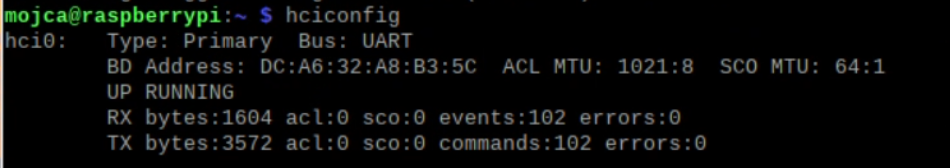
\includegraphics[width=\textwidth]{hciconfig}

\section{Ukaz \textit{hcitool}}
Z ukazom \textit{hcitool scan} pridobimo podatke o napravah v bližini, ki imajo omogočeno Bluetooth povezavo.

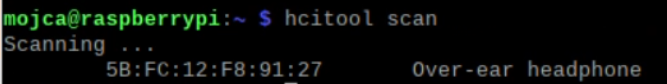
\includegraphics[width=\textwidth]{hcitool}

\section{Ukaz \textit{l2ping}}
Z ukazom \textit{sudo l2ping MAC} smo "pingali" našo napravo 5B:FC:12:F8:91:27, torej v mojem primeru slušalke.

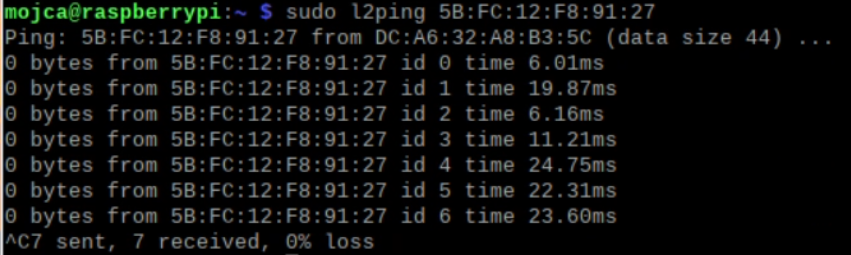
\includegraphics[width=\textwidth]{l2ping}

\section{Zajem prometa z Wiresharok-om}
Z Wireshark-om smo zajeli Bluetooth promet. Zajeli smo nekaj različnih paketov:

\begin{itemize}
	\item Sent Inquiry
	\item Rcvd Command Status
	\item Rcvd Inquiry Complete
	\item Rcvd Extended Inquiry Result
	\item ... (vsi so prikazani na screenshot-u)
\end{itemize}

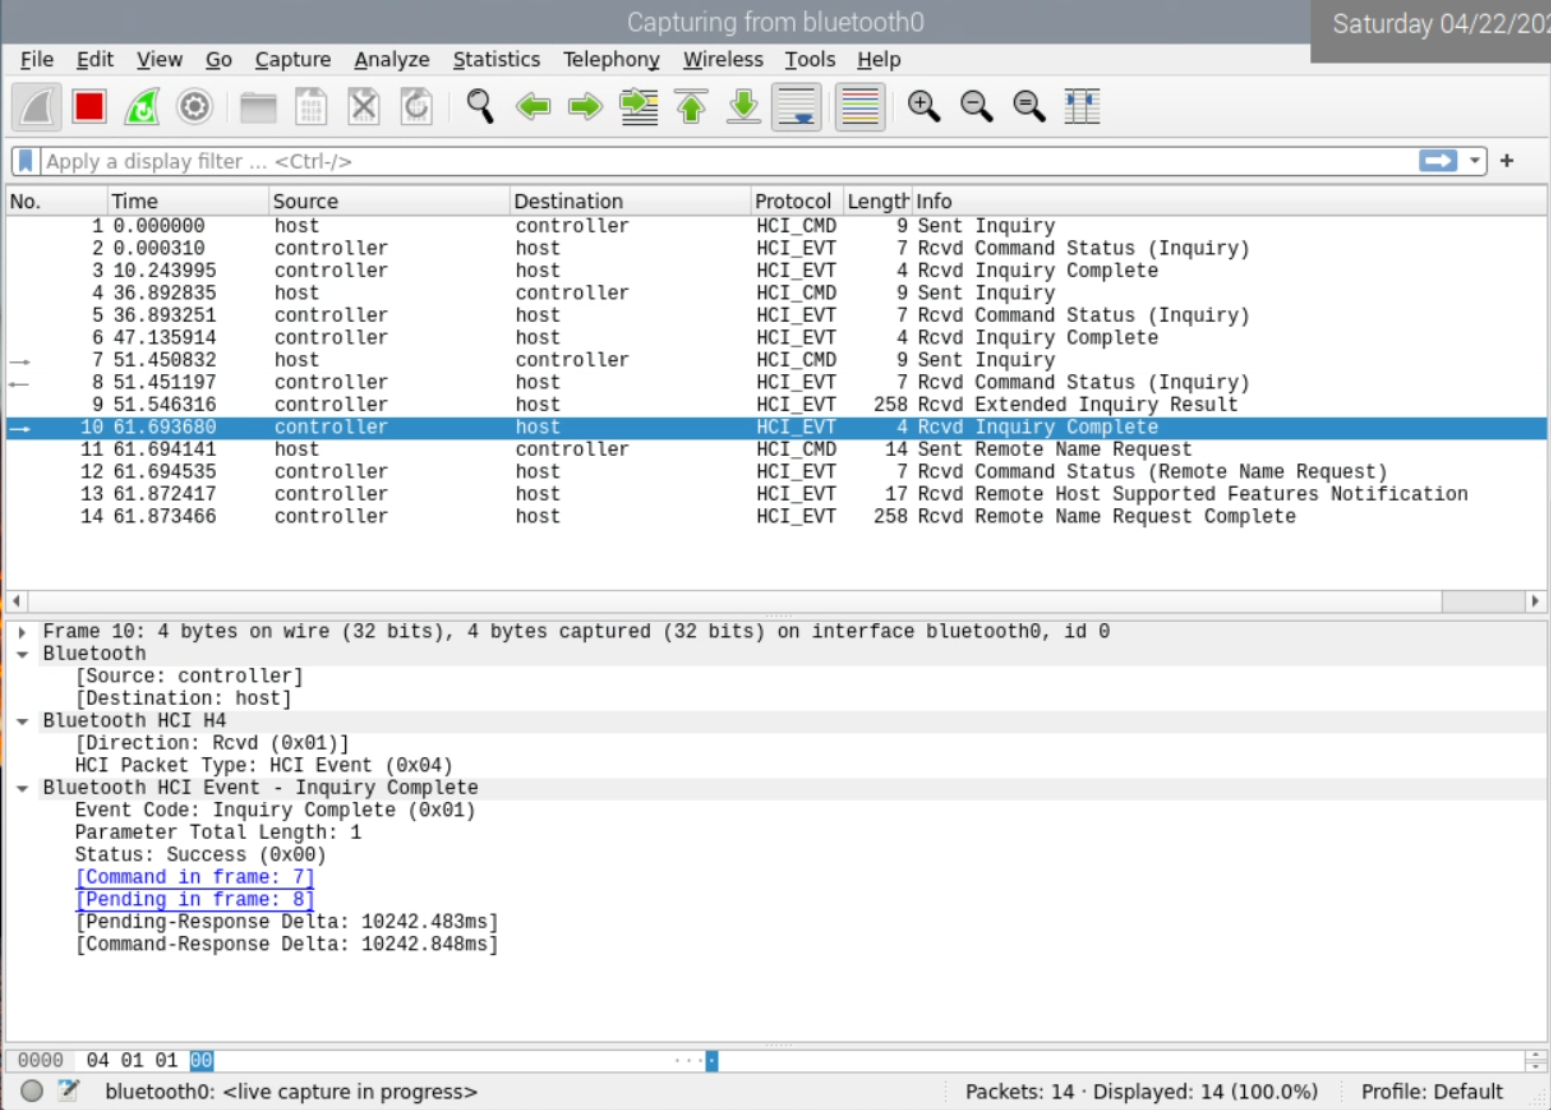
\includegraphics[width=\textwidth]{inquiry_complete}

\pagebreak
\nocite{*}

\end{document}











